\begin{figure*}[h!]
\begin{subfigure}[]{0.27\textwidth}
    \centering
    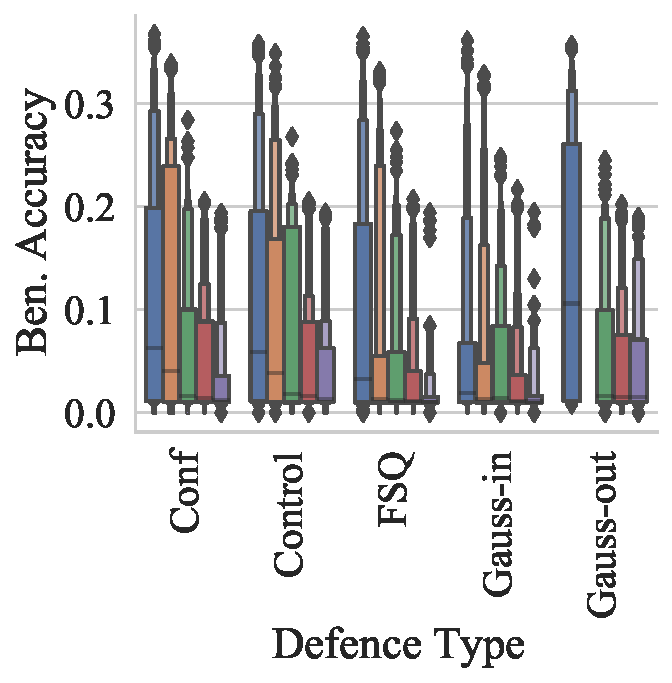
\includegraphics[width=\textwidth]{cifar100/ben_accuracy_vs_defence_type.pdf}
\end{subfigure}
\begin{subfigure}[]{0.27\textwidth}
    \centering
    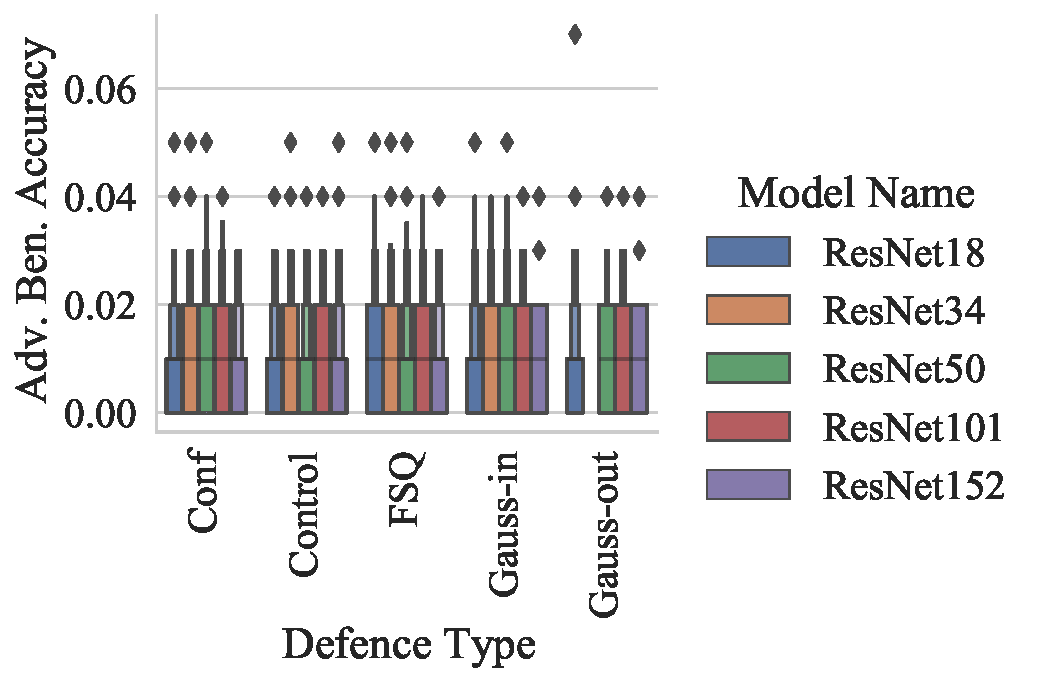
\includegraphics[width=\textwidth]{cifar100/adv_accuracy_vs_defence_type.pdf}
\end{subfigure}
\begin{subfigure}[]{0.36\textwidth}
    \centering
    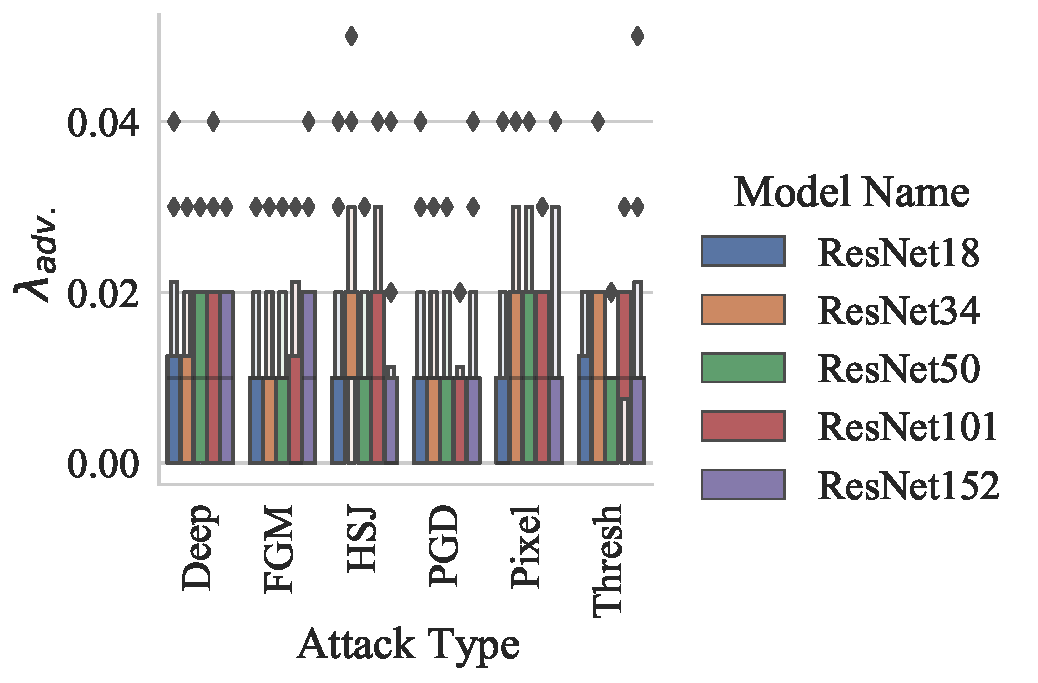
\includegraphics[width=\textwidth]{cifar100/adv_accuracy_vs_attack_type.pdf}
\end{subfigure}
\caption{The adversarial accuracy across various attacks pictured on the x-axis and outlined in Section~\ref{attacks}. The error bar reflects the 95\% confidence interval for the adversarial accuracy across all examined samples.}
\label{fig:cifar100_accuracies}
\end{figure*}

\begin{figure*}[h!]
    \centering
    \begin{subfigure}[]{0.45\textwidth}
        \centering
        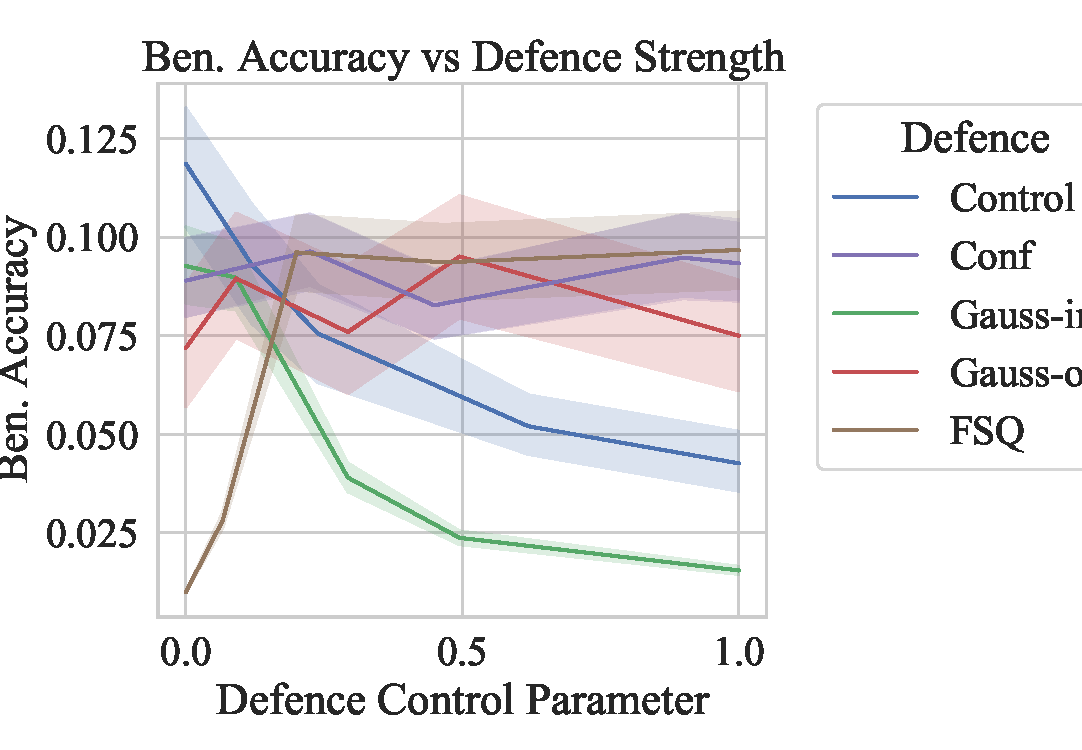
\includegraphics[width=\textwidth]{cifar100/def_param_vs_accuracy.pdf}
    \end{subfigure}
    \begin{subfigure}[]{0.45\textwidth}
        \centering
        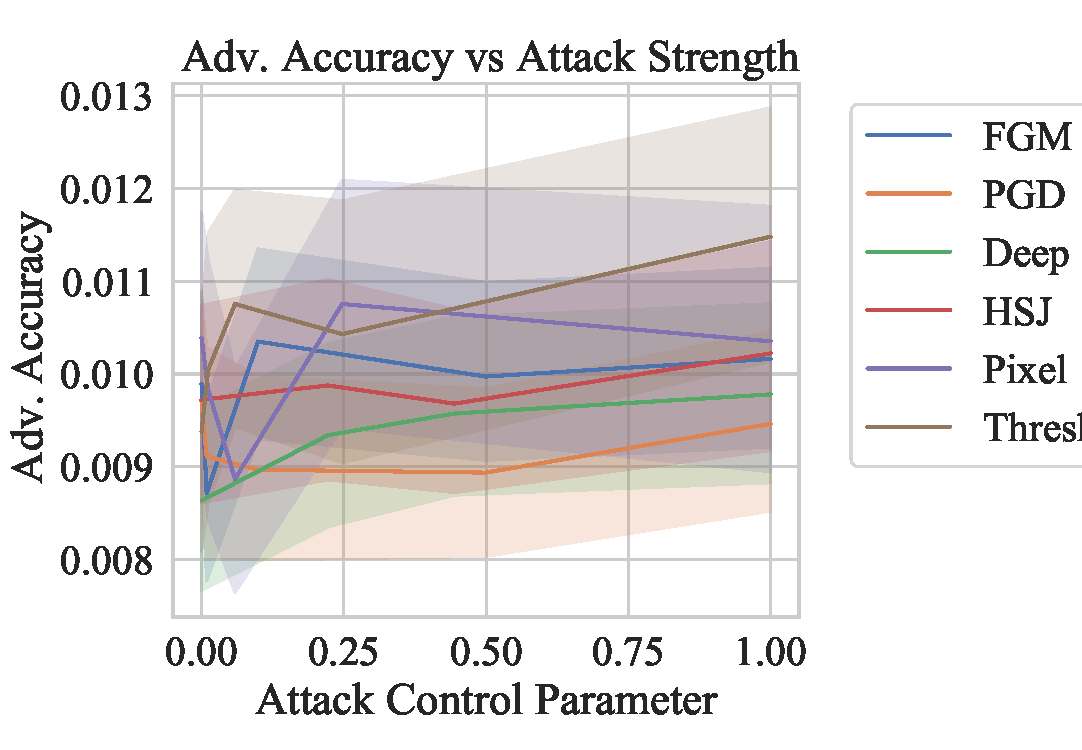
\includegraphics[width=\textwidth]{cifar100/atk_param_vs_accuracy.pdf}
    \end{subfigure}
    \caption{This depicts the benign (unperturbed) and adversarial (perturbed) failure rates across all defences attacks, and models. The left shows how the benign accuracy varies with the defence strength where the control parameter describes the number of layers. The right shows the adversarial accuracy as a function of attack strength.}
    \label{fig:cifar100_strength}
\end{figure*}

\begin{figure*}[h!]
    \begin{subfigure}[]{0.45\textwidth}
        \centering
        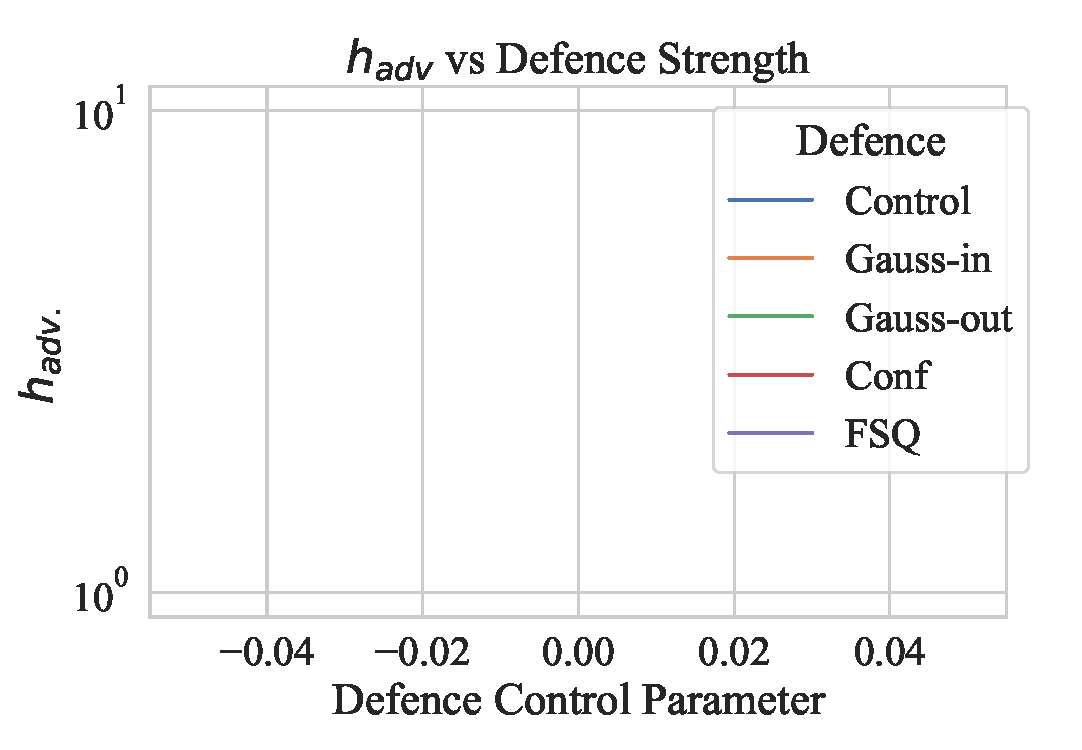
\includegraphics[width=\textwidth]{cifar100/def_param_vs_adv_failure_rate.pdf}
    \end{subfigure}
    \begin{subfigure}[]{0.45\textwidth}
        \centering
        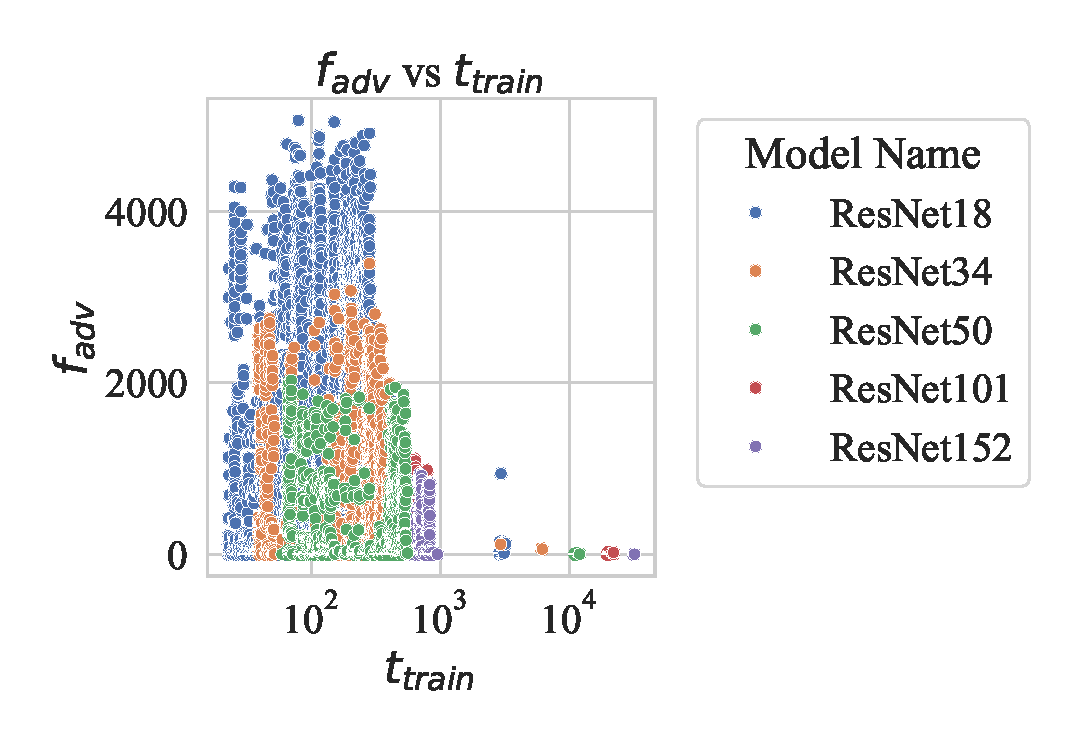
\includegraphics[width=\textwidth]{{cifar100/adv_failure_rate_vs_train_time.pdf}}
    \end{subfigure}
    \caption{The left shows the adversarial failure rate as a function of the defence strength where the control parameter represents the number of model layers. The right depicts the adversarial failure rate as a function of training time and the ResNet configuration.}
    \label{fig:cifar100_failure_rate}
\end{figure*}

\begin{figure*}[h!]
    \centering
    \begin{subfigure}[]{.3\textwidth}
        \centering
        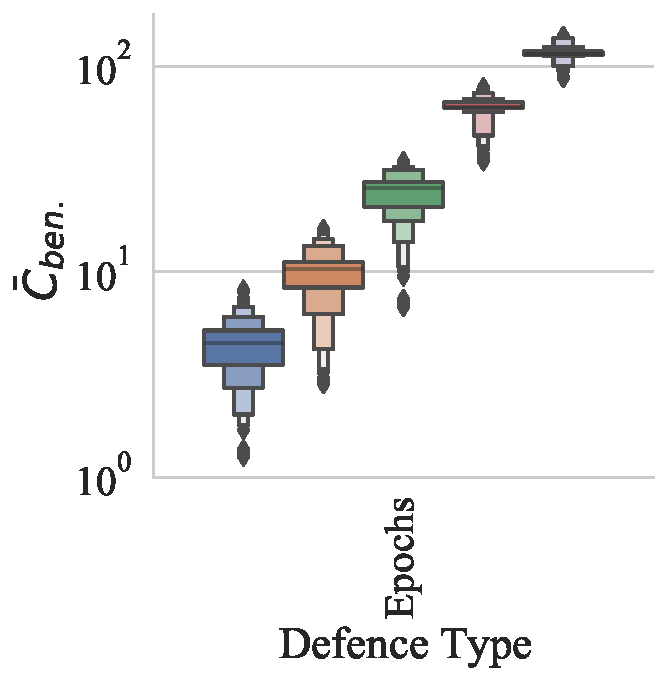
\includegraphics[width=\textwidth]{cifar100/ben_failures_per_train_time_vs_defence_type.pdf}
    \end{subfigure}
    \begin{subfigure}[]{0.3\textwidth}
        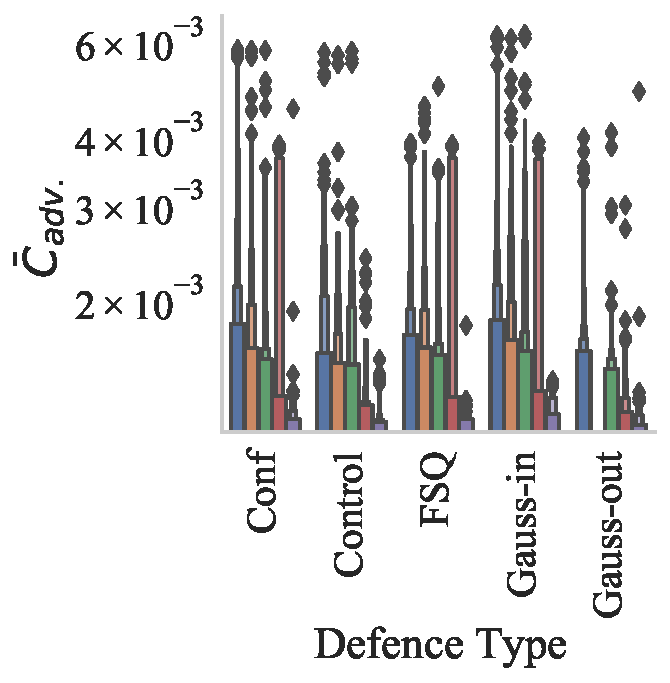
\includegraphics[width=\textwidth]{cifar100/adv_failures_per_train_time_vs_defence_type.pdf}
        \centering
    \end{subfigure}
    \begin{subfigure}[]{0.35\textwidth}
        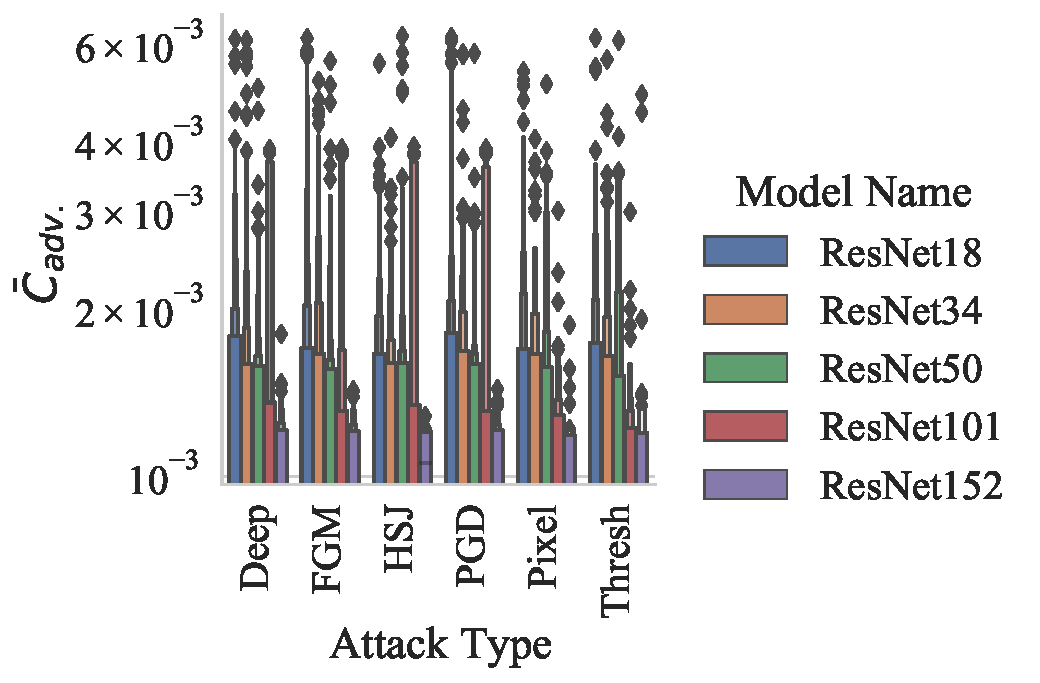
\includegraphics[width=\textwidth]{cifar100/adv_failures_per_train_time_vs_attack_type.pdf}
        \centering
    \end{subfigure}
    \caption{This figure depicts the cost-normalized adversarial failure rate across a variety of defences and attacks, where training time (middle~\&~right Figs.) and inference time (left figure) is a stand-in for cost (see Section~\ref{cost}).}
    \label{fig:cifar100_failures_per_train_time}
\end{figure*}

\begin{figure*}[h!]
    % \centering
    \begin{subfigure}[t]{0.3\textwidth}
        \centering
        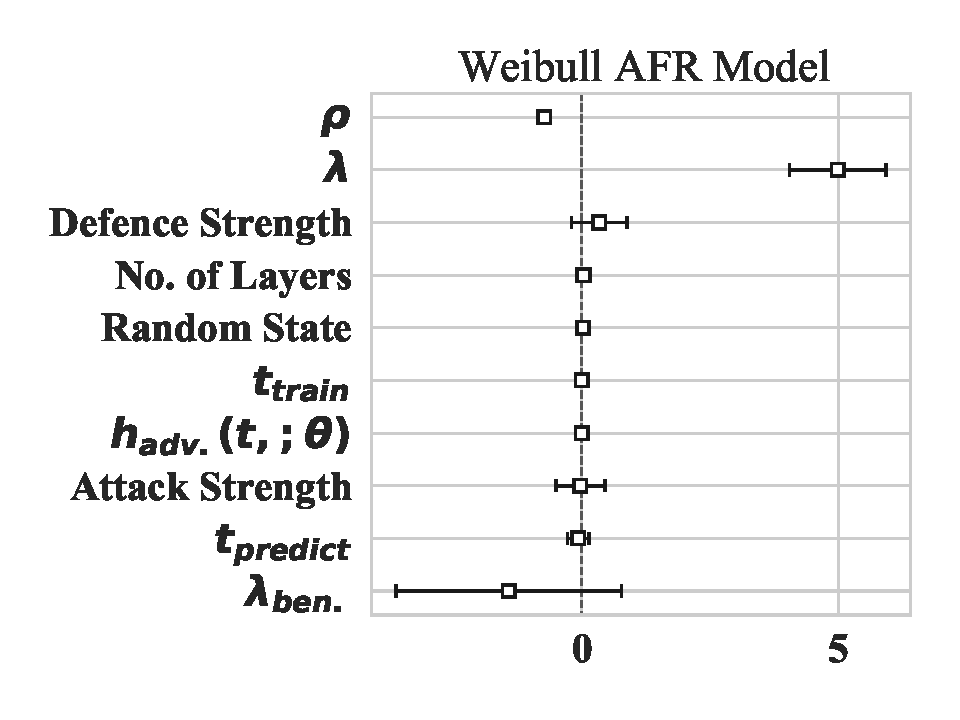
\includegraphics[width=\textwidth]{cifar100/weibull_aft.pdf}
    \end{subfigure}%
    ~ 
    \begin{subfigure}[t]{0.3\textwidth}
        \centering
        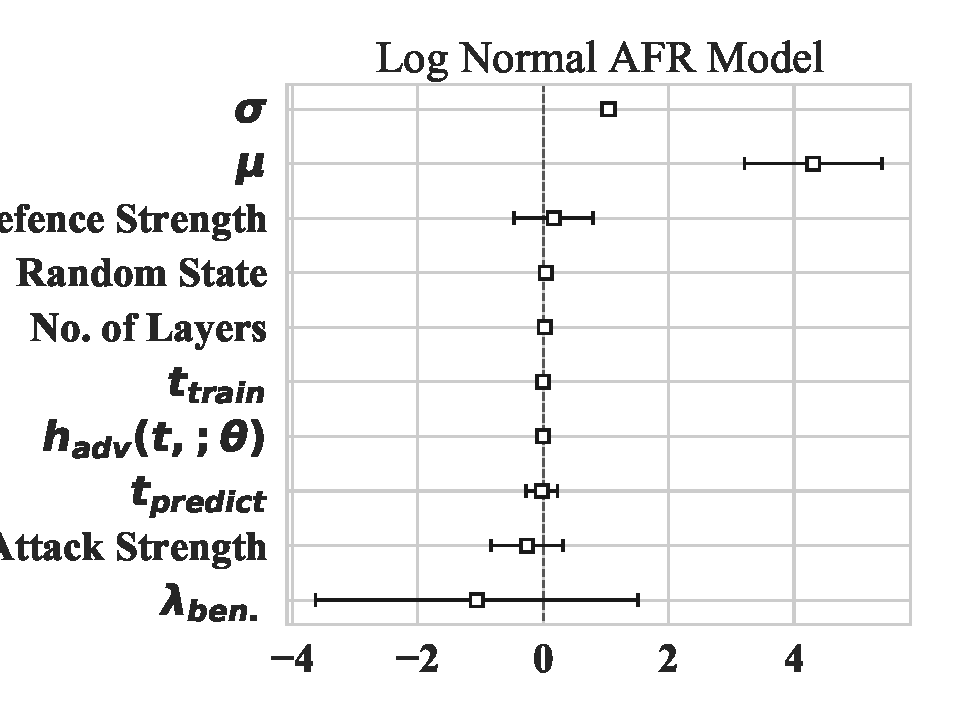
\includegraphics[width=\textwidth]{cifar100/log_normal_aft.pdf}
    \end{subfigure}
    ~
    \begin{subfigure}[t]{0.3\textwidth}
        \centering
        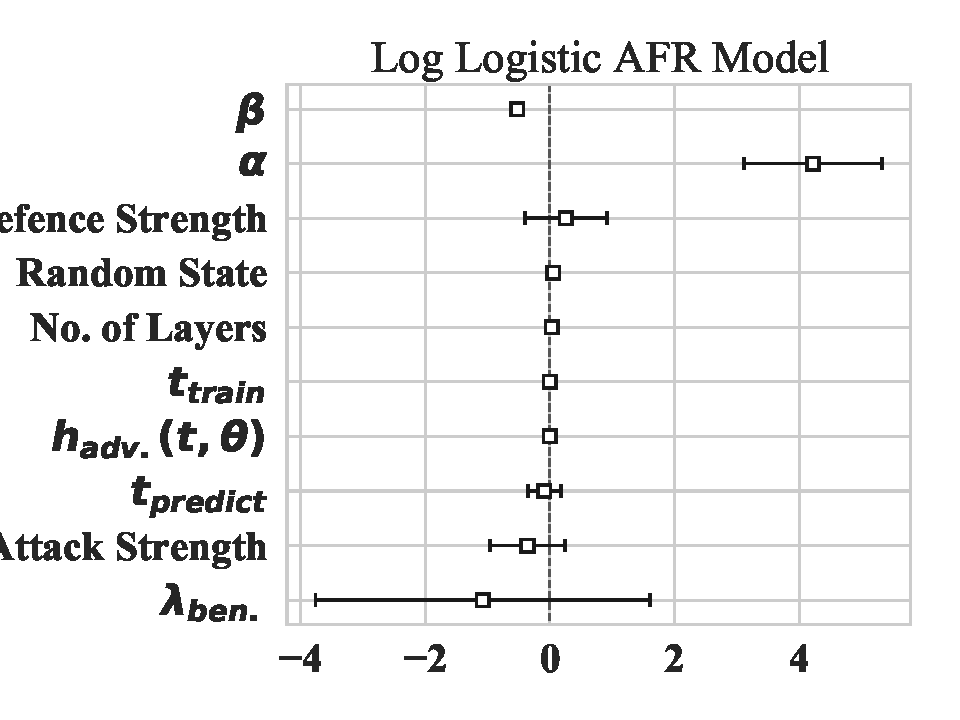
\includegraphics[width=\textwidth]{cifar100/log_logistic_aft.pdf}
    \end{subfigure}
    
    \caption{The covariate estimates accelerated failure time models where the parameters $\rho$, $\lambda$, $\mu$, $\sigma$, $\alpha$, and $\beta$ represent the intercepts for those parameters as described in Section~\ref{afr_models} for the Weibull, Log-Normal, and Log-Logistic AFR Models. The coefficients represent the log scale effect of the covariates on the failure rate.}
    \label{fig:cifar100_afr_models}
\end{figure*}

\begin{figure}[h!]
    \centering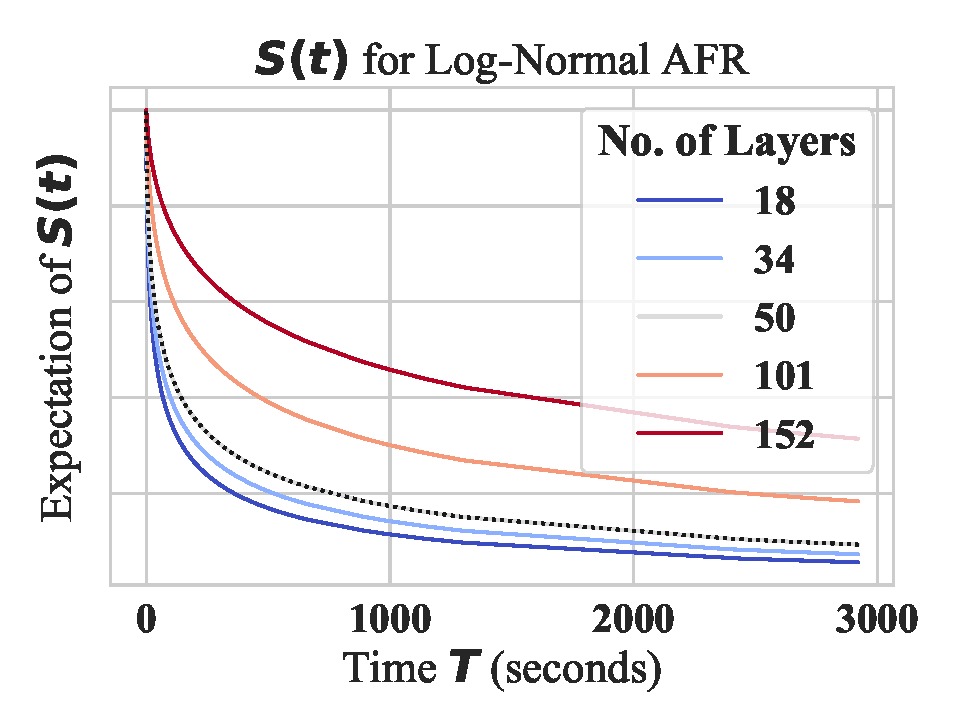
\includegraphics[width=.5\textwidth]{cifar100/log_normal_partial_effects.pdf}
    \caption{This figure depicts the survival curve over time as a function of the number of model layers for the highest scoring model (the Log-Normal distribution). The partial effects plots of other models were excluded for space reasons, but the results were nearly identical.}
    \label{fig:cifar100_cifar100_layers}
\end{figure}
\begin{table}
\centering
\caption{Comparison of AFR Models on the CIFAR100 dataset.}
\label{tab:cifar100}
\begin{tabular}{lrrrrr}
\toprule
{} &      AIC &  Concordance &      BIC &  Mean \$S(t;\textbackslash theta)\$ &  Median \$S(t;\textbackslash theta)\$ \\
\midrule
Weibull      & 4.76e+03 &        0.848 & 4.76e+03 &                19.9 &                  4.12 \\
Log logistic &  4.7e+03 &        0.856 &  4.7e+03 &                15.3 &                  3.97 \\
Log normal   & 4.76e+03 &        0.855 & 4.76e+03 &                16.7 &                  3.93 \\
\bottomrule
\end{tabular}
\end{table}
